\documentclass[12pt,a4paper]{article}

\usepackage[brazil]{babel}
\usepackage[utf8]{inputenc}
\usepackage{geometry}
\usepackage{amssymb}
\usepackage{amsmath}
\usepackage{amssymb}
\usepackage{amsfonts}
\usepackage{fancyhdr}
\usepackage{epsfig}
\usepackage{multirow}
\usepackage{graphicx}
\usepackage{setspace}
\usepackage{makeidx}
\usepackage{caption}
\usepackage{subcaption}
\usepackage{algorithm}
\usepackage{algpseudocode}
\usepackage{xspace}
\usepackage[linktocpage=true]{hyperref}

% \geometry{
%     a4paper,
%     total={210mm,297mm},
%     left=20mm,
%     right=20mm,
%     top=20mm,
%     bottom=20mm,
% }

\begin{document}

\title{Relatório do Trabalho de Fundamentos Lógicos da Inteligência Artificial}
\author{Eduardo Luis Buratti}
\date{\today}

\maketitle

\section{Introdução}

Em \cite{skliarova2004reconfigurablehardware}, é feito um levantamento de todas as implementações de resolvedores SAT em hardware (usando FPGAs). Analisando todas as soluções apresentadas, foi escolhido implementar uma solução baseada em Zhong et al. \cite{zhong1998usingreconfigurable}, visto que é uma das mais simples e também essa implementação serviu de base para o trabalho de outros que vieram na sequência.

Este relatório apresenta na Seção \ref{sec:rev} uma breve revisão da bibliografia da área. Na Seção \ref{sec:exp} são expostos alguns experimentos realizados, comparando a solução em hardware com outras em software.

\section{Revisão Bibliográfica}
\label{sec:rev}

A idéia de implementar um resolvedor SAT em hardware vem desde 1996 com o artigo do Suyama et al. \cite{suyama1996solvingsatisfiability}. Neste, dada uma instância SAT, é gerado um código VHDL correspondente que é compilado e aplicado à uma FPGA que executa o circuito e resolve a instância. Essa abordagem é denominada \textit{instance-specific}, pois o código HDL gerado é específico aquela instância. A Figura ? representa uma visão geral de como ocorre o processo de um resolvedor \textit{instance-specific} em hardware.

A abordagem proposta por Suyama et al. \cite{suyama1996solvingsatisfiability} pode ser vista na Figura \ref{fig:suyama}. A cada ciclo de \textit{clock}, todas as váriaveis são testadas com todas as claúsulas ao mesmo tempo e então é feito o \textit{backtracking} ou \textit{branching} dependendo da existência ou não de conflitos. O problema é que desta forma o circuito fica imensamente grande e utiliza mal os recursos das FPGAs.

\begin{figure}[H]
    \centering
    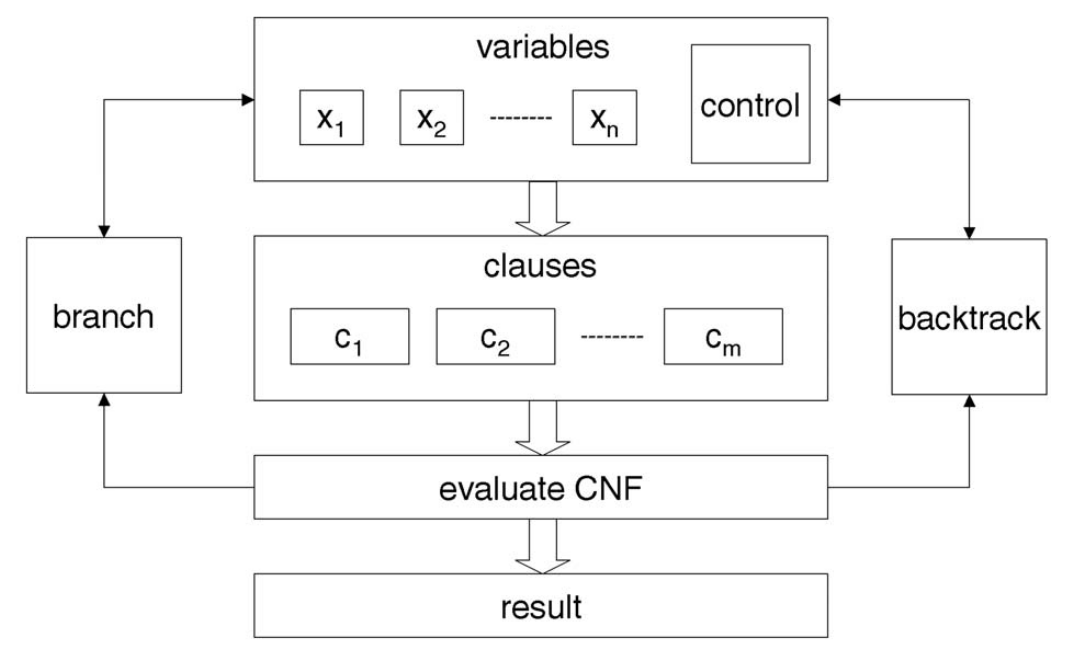
\includegraphics[width=0.7\textwidth]{figures/suyama}
    \caption{Visão geral da solução proposta por Suyama et al. Fonte: \cite{skliarova2004reconfigurablehardware}.}
    \label{fig:suyama}
\end{figure}

Em 1998, Zhong et al. \cite{zhong1998usingreconfigurable}, propuseram uma maneira mais interessante de implementação. Neste, a representação de cada variável é feita por 2 bits. Se ambos são 0, a varíavel não tem nenhum valor definido (variável livre). Se o primeiro bit for 1 e o segundo 0, a variável é verdadeira. Se os bits forem 0 e 1 respectivamente, a variável é falsa. E, finalmente, quando ambos os bits são 1, isso denota um conflito (a váriavel é verdadeira e falsa ao mesmo tempo). De forma mais simples, é possível pensar na representação como uma tupla $(a, \lnot a)$ para uma váriavel qualquer $a$, onde os elementos da tupla são bits.

Cada váriavel da fórmula de entrada é representada por uma máquina de estados finita e um circuito de implicação. Este último é análogo à propagação unitária no DPLL. Para cada variável é construído um circuito que representa as possíveis valorações para as outras variáveis que implicam o valor verdadeiro para a variável em questão (e também um circuito para as que implicam o valor falso). Uma representação do circuito para a váriavel $a$ na fórmula $(\lnot c \vee a) \wedge (\lnot d \vee a) \wedge (\lnot b \vee c \vee a) \wedge (e \vee \lnot a) \wedge (c \vee \lnot a)$ pode ser vista na Figura \ref{fig:imp}. A váriavel $a$ é implicada verdadeira por $c \vee d \vee (b \wedge \lnot c)$ e implicada falsa por $\lnot e \vee \lnot c$.

\begin{figure}[H]
    \centering
    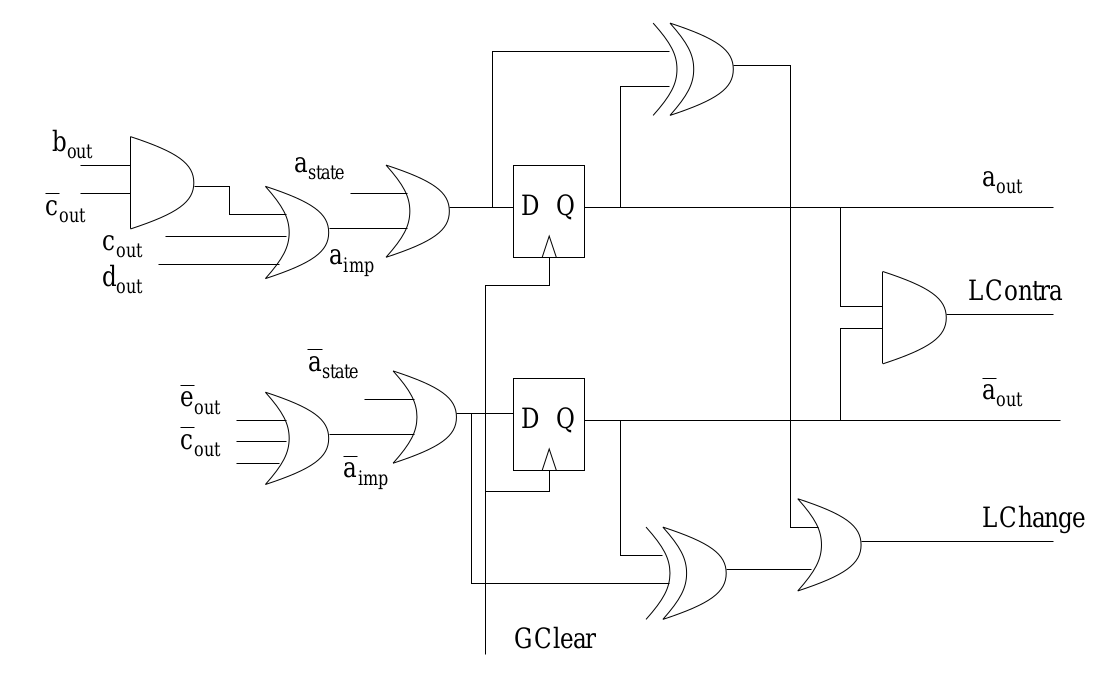
\includegraphics[width=0.7\textwidth]{figures/imp}
    \caption{Circuito de implicação da variável $a$. Fonte: \cite{zhong1998usingreconfigurable}.}
    \label{fig:imp}
\end{figure}

A representação da máquina de estados para uma variável pode ser vista na Figura \ref{fig:fsm}. Em um determinado momento, somente a máquina de estados de uma única variável pode estar no estado ativo (as outras estão em estado de espera), significando que esta variável está sendo decicida. E quando uma váriavel está sendo decicida, o circuito de implicação de todas as variáveis é ativado. Se algum conflito for detectado, faz-se \textit{backtracking} (simplesmente passando o estado ativo para a váriavel anterior). Senão, a busca continua passando o estado ativo para a variável seguinte (mantendo o valor das variáveis que foram implicadas pelos circuitos de implicação).

\begin{figure}[H]
    \centering
    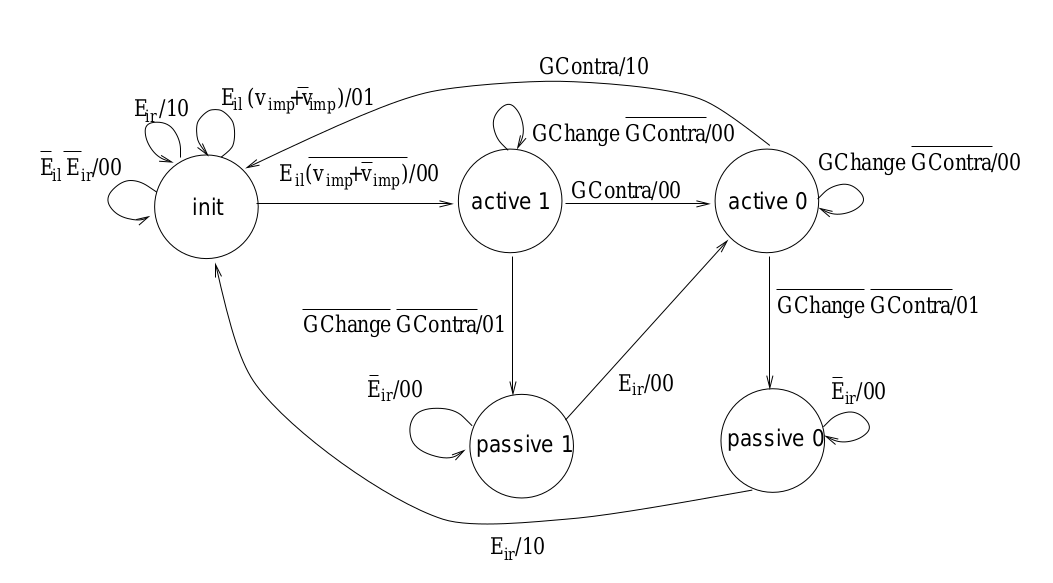
\includegraphics[width=0.7\textwidth]{figures/fsm}
    \caption{Máquina de estados da variável $a$. Fonte: \cite{zhong1998usingreconfigurable}.}
    \label{fig:fsm}
\end{figure}

Mais a frente, Dandalis et al. \cite{dandalis2002runtimeperformance} propõe uma melhor organização e compartimentalização do circuito, no qual a formúla de entrada é divivida em subfórmulas e durante a execução são feitos \textit{merges} com uma frequência constante. Em \cite{skilarova2004asoftware}, Skilarova et al. utilizam uma estratégia \textit{application-specific} (não mais \textit{instance-specific}), ou seja, o resolvedor já compilado e em funcionamento na FPGA é que recebe a fórmula em CNF (não há o passo de gerar código específico para a instância de entrada).

\section{Experimentos}
\label{sec:exp}

Neste trabalho, foi implementado a solução do Zhong et al \cite{zhong1998usingreconfigurable}. Um programa em Python recebe a fórmula CNF (no formato DIMACS) e, a partir de \textit{templates}, gera o código em VHDL correspondente. Para testes, o simulador GHDL compila o código e gera um programa que ao ser executado simula a execução do circuito. Os experimentos foram executados em um computador com um processador ``AMD FX(tm)-8120 Eight-Core Processor'' de 3,1 GHz, 8 GiB de memória e todo o código está disponível no repositório \url{https://github.com/bazk/hwsat}.

As figuras \ref{fig:ram-nocomp} e \ref{fig:hole-nocomp} demonstrar o tempo de execução para um total de 7 instâncias dentre utilizadas para teste.
As instâncias \textit{ram6} e \textit{ram8} são satisfasíveis, enquanto as instâncias \textit{ram10}, \textit{ram12}, \textit{hole6}, \textit{hole7} e \textit{hole8} são insatisfasíveis. Nos gráficos, a implementação deste trabalho é representada por \textbf{zhong}.

\begin{figure}[H]
    \centering
    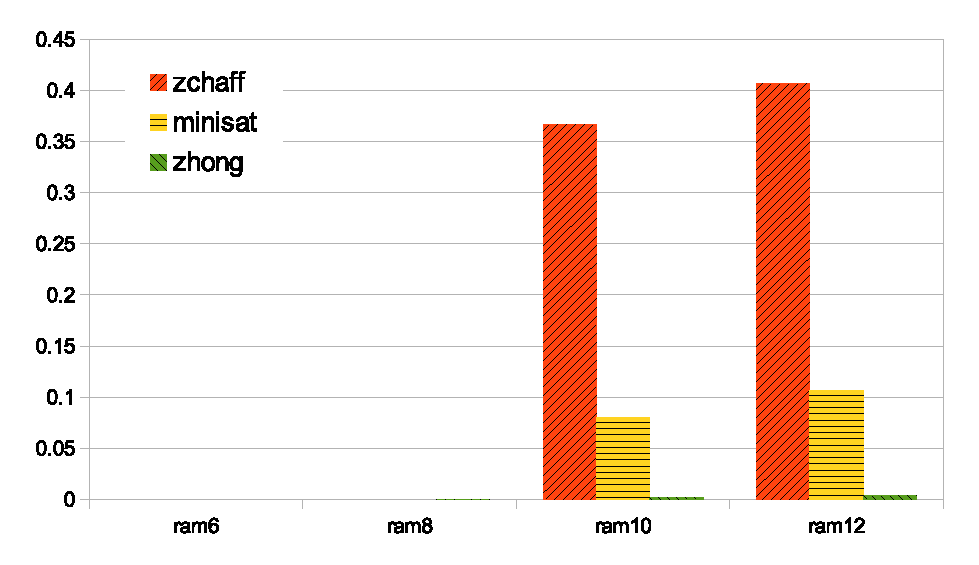
\includegraphics[width=0.7\textwidth]{figures/ram-nocomp}
    \caption{ram nocomp}
    \label{fig:ram-nocomp}
\end{figure}

\begin{figure}[H]
    \centering
    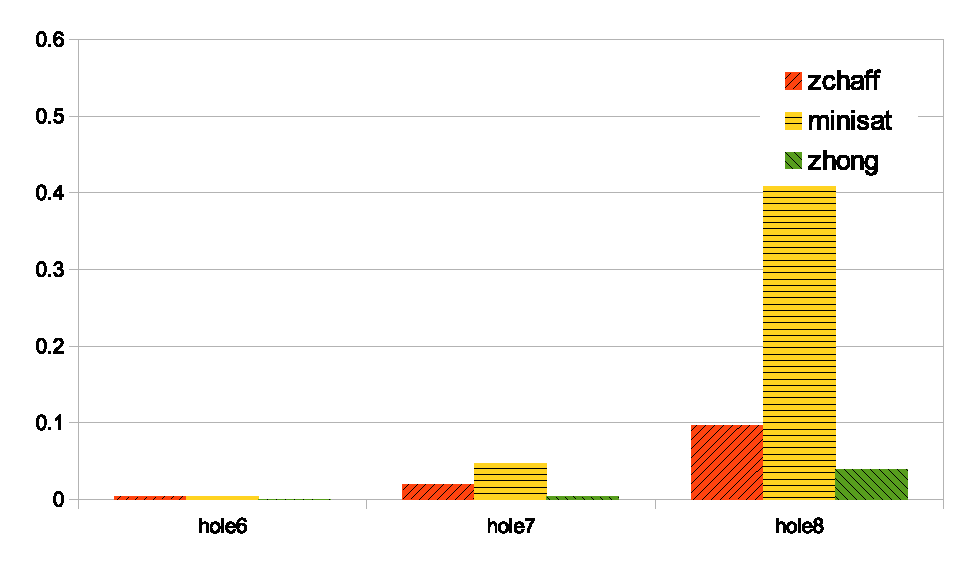
\includegraphics[width=0.7\textwidth]{figures/hole-nocomp}
    \caption{hole nocomp}
    \label{fig:hole-nocomp}
\end{figure}

Percebe-se que o tempo de execução em hardware é menor do que os algoritmos de referência implementados em software. Porém, não foi contado o tempo de compilação. Nas figuras \ref{fig:ram-comp} e \ref{fig:hole-comp} é mostrado o tempo de execução somado do tempo de compilação para as mesmas instâncias de antes. Agora, a implementação em hardware é muito mais ineficiente e chega a ser pior do que o algoritmo GRASP.

\begin{figure}[H]
    \centering
    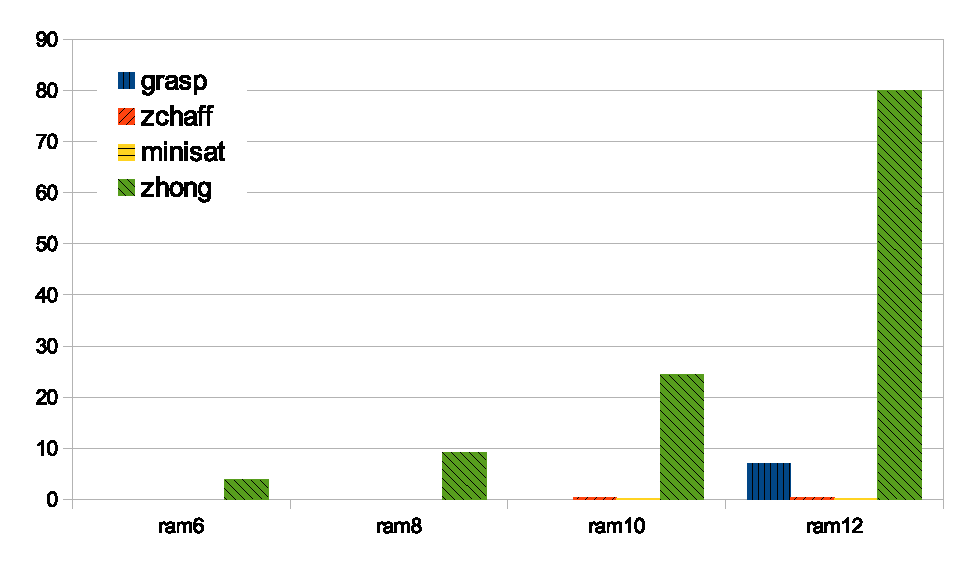
\includegraphics[width=0.7\textwidth]{figures/ram-comp}
    \caption{ram comp}
    \label{fig:ram-comp}
\end{figure}

\begin{figure}[H]
    \centering
    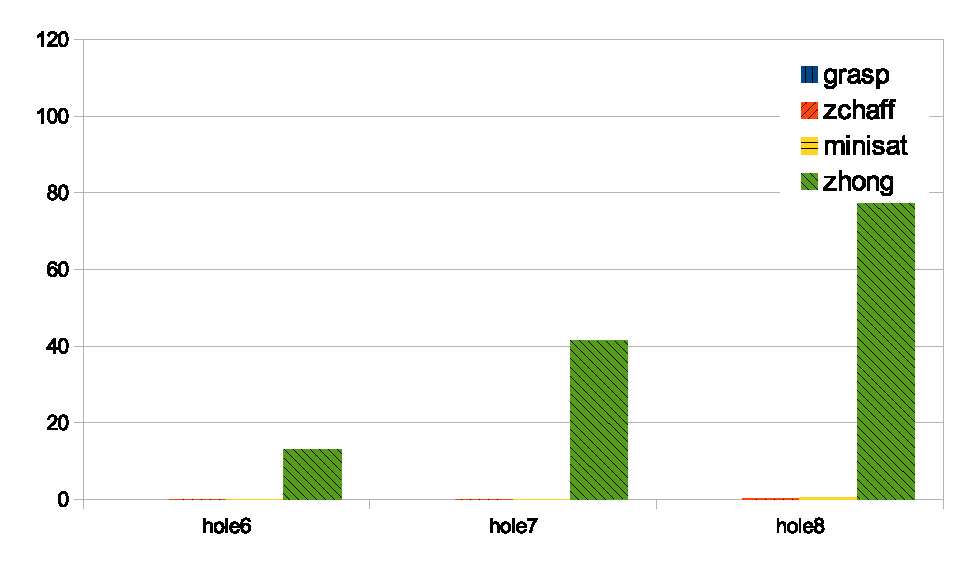
\includegraphics[width=0.7\textwidth]{figures/hole-comp}
    \caption{hole comp}
    \label{fig:hole-comp}
\end{figure}

\section{Conclusão}

O tempo de compilação dos resolvedores \textit{instance-specific} em hardware tornam esse tipo de solução inviável (porque hoje existem resolvedores eficientes em software). Para um número grande de variáveis, o tempo de compilação pode chegar a horas. Ainda assim, historicamente é interessante observar a evolução de tais soluções em uma época em que os resolvedores em software ainda não eram tão eficientes.

Os resolvedores \textit{application-specific} já são comparáveis aos resolvedores em software. Porém, sua complexidade de implementação e a necessidade de um hardware adicional (uma FPGA) acabam não justificando os ganhos de performance destas soluções.

\bibliographystyle{plain}
\bibliography{referencias}

\end{document}
